\chapter{Hands On Analysis of BLE traffic}
\label{chapter3}
\thispagestyle{empty}

\noindent 
This chapter is dedicated to BLE traffic analysis between two BLE devices.
In the first case we used a phone and a smart bulb, in the second case a phone (in either cases even a laptop is fine) and a STM IoT Node.
In particular we used a Magic Blue smart bulb that had it's own application, downloadable from the App Store, and Wireshark 2.6.2 software. As this tool is unable to sniff BLE packets unless another support is provided (like Ubertooth or Nordic Semiconductor dongle), we decided to use the phone Developers Option's tool to register incoming and outgoing Bluetooth traffic.
Through this setting, it becomes easy to track all the packets from the phone to the smart bulb in a single log file. Wireshark provides an interface to read it in a comprehensible and user-friendly way.
The STM Iot Node we used is the B-L475E-IOT1A2 Discovery kit with integrated BLE module, with the Mbed Online Compiler support.

\section{Hacking a smart bulb through BLE}
\subsection{Connect to the device}

The first step in order to sniff packets from a device is to know its bluetooth address and understand how its profile is structured.
Many tools are available, just to mention the ones we employed, Hcitool, Bluetoothctl and Gatttool.

These three programs are just an example of what the Bluez stack offers: it is the official Linux Bluetooth Protocol and provides support to the user for Bluetooth Layers and Protocols.
Due to its modularity, it is easy to install just the modules and libraries that are needed, and quickly get to work with devices.

They all provide similar functions and the choice is really up to the user. In this case of study, the main objective was to scan the surroundings for BLE and BT devices and to connect to them and gather more informations about their services and characteristics.

Following, are the command lines to scan and connect to the devices.

\lstinputlisting{lescan-connect.txt}
\lstinputlisting{bluetoothctl-connect.txt}
\lstinputlisting{gatttool-connect.txt}

Our choice on which tool to use, fell on Gatttool, simply due to its efficiency in displaying the characteristics and services of a certain device. That is why in the following explanation only Gatttool will be taken into account.
Through some simple commands, once the connection has been achieved, it is possible to explore the characteristics (all of them or only the primary ones) of the device.

\lstinputlisting{gatttool-characteristics.txt}

However, as the code shows, it is impossible to understand the meaning and purpose of each characteristics, and in this case, even the Bluetooth GATT Services table does not provide much support.

Another way to connect to the device may be through a BLE sniffer app, like BLEScanner or nRFConnect.
Turn the Bluetooth on, and in the main page connectible devices appear: the user can then easily open another tab and explore the content more deeply.

\begin{figure}
	\centering
		\includegraphics[width=0.9\textwidth]{0.5\textwidth}
	\label{fig:images\nrfConnect}
\end{figure}	

Although all the services appear as unknown and it is not clear the meaning of the values, the structure of the device profile, including characteristics, services and descriptors is apparent.
At this point it is understandable that only knowing the characteristics and services of a device is not sufficient to understand what the data sent from the phone to the smart bulb is. There is a tool in every smart phone (from Android 4.0 onwards) that allow users to capture all Bluetooth HCI packets in a file, called HCI snoop log, and it is accessible from the Developer Option section in the system Settings. It is important to take into account that this section is not usually available and it has to be activated direclty from the user.

The next step is to connect to the MagicBlue app and select the smart bulb. From here it is possible to choose from a range of colours and modes, modify the brightness and the interval of time between the lights, as well as enable the microphone sensitivity or play music from the phone and light up the bulb according to it.
By doing these operations, the phone sends to the bulb data packets containing the command requests for the bulb, and  all this information is recorded in a snoop log file.
After transferring the file from the phone to a PC, Wireshark is the instrument needed to read from the log file.

\subsection {Filtering}
One of the obstacles in understanding the structure of data packets exchanged between two BLE devices is finding the packets of interest. The amount of data gathered in the log file is indeed impressive, but many of the packets are related to the connection phase between the two entities and  in this case they hold no value for our research.
It is thus advisable to use as a filter(there is a specific bar in Wireshark to do this) on the Bluetooth address of the device, acquired during the initial scanning phase.

After this step, only the packets sent from and to the smart bulb remain. Wireshark provides a complete description of the packets and, while at the beginning it may seem impossible to decipher the values of the data exchanged, it is then quite easy to spot recurring similarities.

\begin{figure}
	\centering
	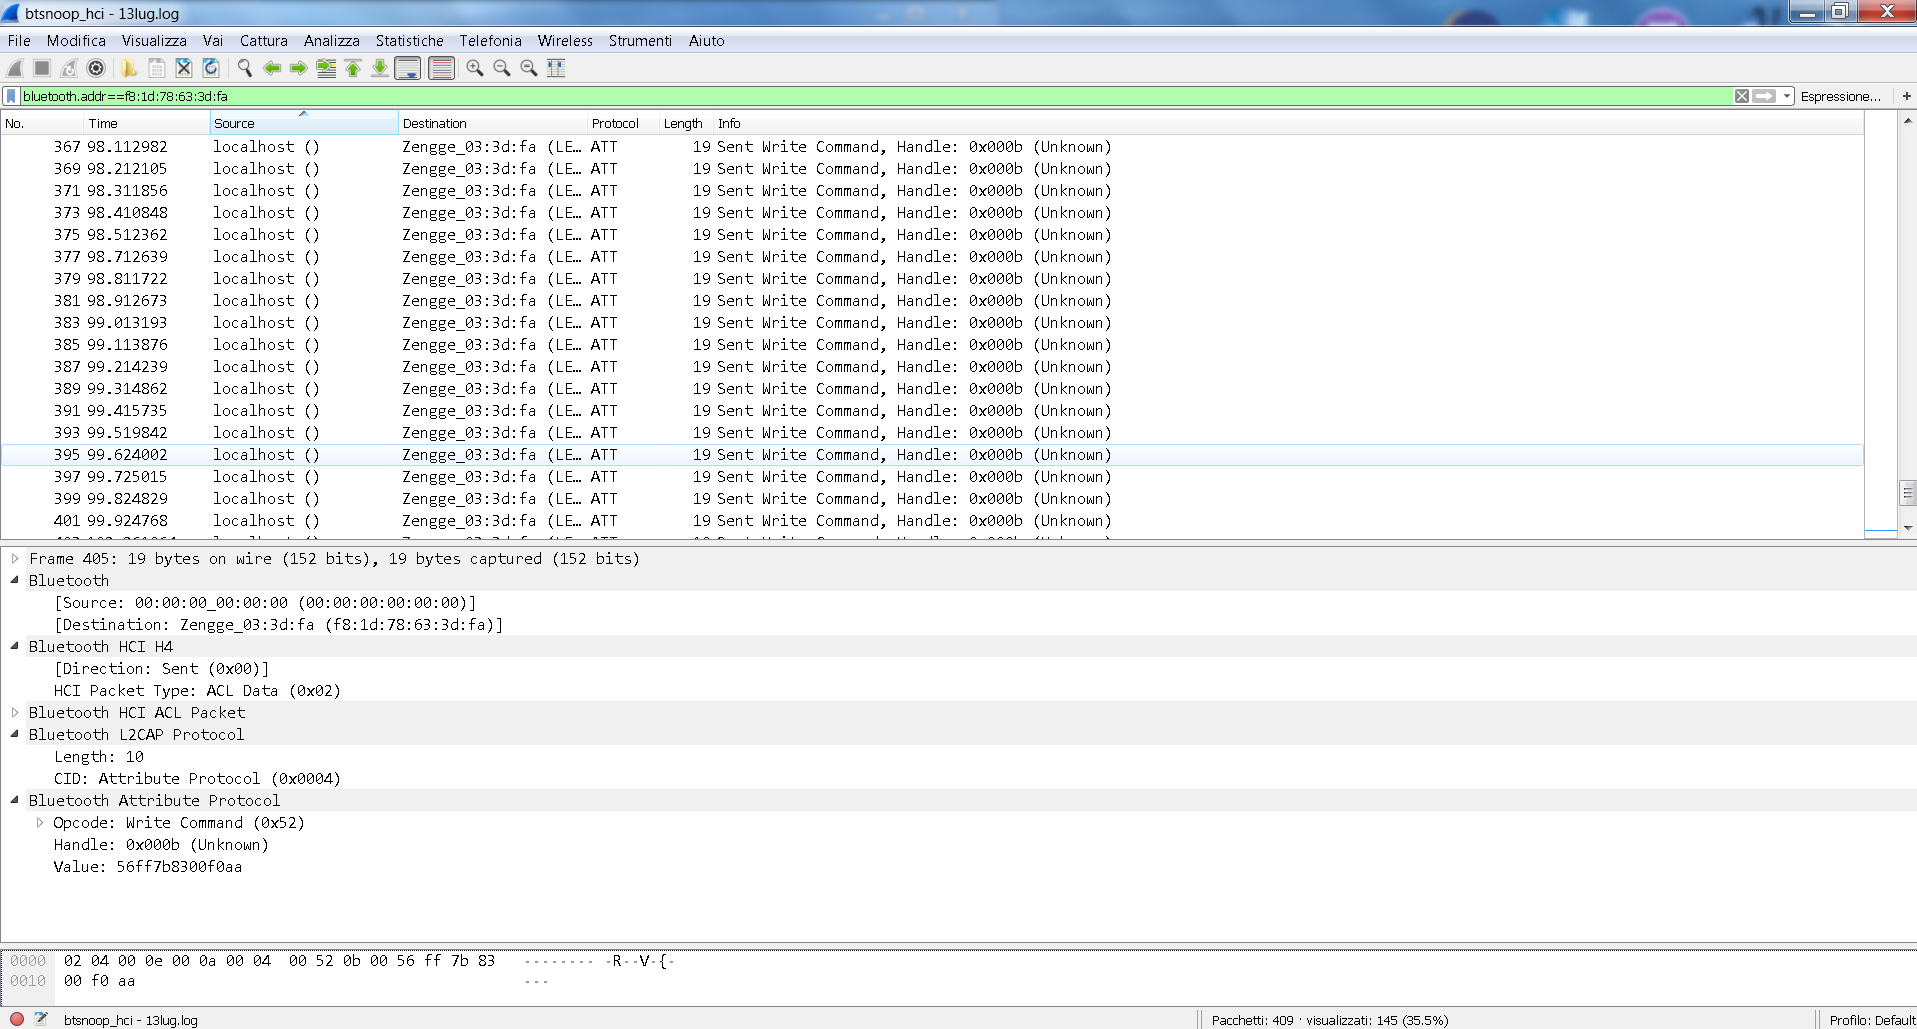
\includegraphics[width=0.9\textwidth]{wireshark1}
	\label{fig:images\wireshark1}
\end{figure}

Through data packets analysis, patterns are recognized and it becomes easy to guess the combination for colour changes and different modes. Following, a partial and brief summary of what we were able to gather from Wireshark log.

\begin{itemize}
	\item Value length is not fixed, up to a maximum of 20 bytes, depending on the information it stores.
	\item Writeable Characteristics are usually marked with a ffe9-XX UUID, referring to a ffe5-XX Service.
	\item There are no security layers and it is possible to write values as one wishes.
	\item It is extremely easy to do so either through a terminal using Gatttool or Bluetoothctl specific commands, or through a BLE sniffer app.
\end{itemize}
-------> DEVO METTERE LE IMMAGINI ANCHE QUI??

Following, the patterns we were able to recognize from the smart bulb MagicBlue.

\textit{Single colour choice example}
\begin{itemize}
	\item 56: fixed prefix.
	\item ff085a: colour RGB code.
	\item 00: from 00 to ff, brightness of the light.
	\item 0f: or f0, off/on.
	\item aa: fixed suffix.
\end{itemize}

\textit{Light Functions example}
\begin{itemize}
	\item bb: fixed prefix.
	\item 3: or 2, respectively for "strobo" or "gradual change"
	\item 0: from 0 to c, 7 colours mode, red, green, .. , white mode.
	\item 1: on-time of the light (1 is a flash, f lights up the led for 5 seconds).
	\item f: interval of time between flashes (1 faster than f).
	\item 44: fixed suffix.
	
There are also other functions and modes but the deciphering of the packets is indeed quite strenuous. 
Hacking a smart bulb may be also accomplished by writing a Python script and compile it on a Raspberry device or other devices that support an operative system. It is in fact needed to install Bluez components, in addition to a code compiler.
This way, controlling the device remotely and in a continued way would be possible.
There is a full Python Compiler called MicroPython for STM Microcontrollers but it did not provide compatibility for the board we used in this project.
The list of supported boards is available from the official site.
	
\section{STM Iot Node advertising test}
 
For this experiment, we used the STM IoT node and tested it on both our Linux distributions. The board retrieves the temperature and humidity levels in the environment and broadcasts them as a non-connectable advertising packet, as we can see in Listing \ref{list:adv-temp-hum}.
\lstinputlisting[caption={Retrieve sensor values and update packet},label={list:adv-temp-hum},language=c++]{example-temphum.cpp}

Packets broadcasted by the board can be retrieved with any of the tools described at the end of the previous chapter. We analysed the payload and found that it follows this structure:
\begin{center}
	\textit{length - meaning - content}.
\end{center}
The length is expressed in bytes and it refers to the overall size of \textit{meaning} and \textit{content}. The former two is a label which has to be matched with the corresponding Bluetooth GAP Assigned Number (specification available on the website, we report the table in Appendix \ref{appendixA}) to understand its meaning. Common examples are \texttt{0x09} for "Complete Local Name" or \texttt{0x0a} for "Power Level". In our case, the label corresponds to "Service data 16-bit UUID", which means that we should look at the next two bytes to have a more precise indication of the received data. Vendors usually publish a web page in which they list all their codes with the respective meaning, while in this example we can see that its value is added to the payload in \texttt{service\_data[0]}, and corresponds to \texttt{00 aa}.

Finally, the next two bytes encode the temperature and humidity in the room.

